% ---------------------------------------------------------------------------
% Device icons for network and process schematics (TikZ pics).
% Every icon is drawn around its origin and is wrapped in a node so that
% connectors attach to the node's anchors (north, south, east, west ...).
% Usage:  \node[dev] (a) at (0,0) {\devserver};   then  \draw (a) -- (b);
% ---------------------------------------------------------------------------
\usetikzlibrary{positioning,arrows.meta,calc,fit,backgrounds,shapes.geometric,shapes.symbols,shapes.misc,decorations.pathreplacing}

\definecolor{devline}{HTML}{37474F}
\definecolor{devfill}{HTML}{ECEFF1}
\definecolor{devacc}{HTML}{1E88E5}
\definecolor{devgreen}{HTML}{43A047}
\definecolor{devred}{HTML}{E53935}
\definecolor{devamber}{HTML}{FB8C00}
\definecolor{devpurple}{HTML}{8E24AA}
\definecolor{zonedata}{HTML}{E3F2FD}
\definecolor{zonectl}{HTML}{FFF3E0}
\definecolor{zoneusr}{HTML}{E8F5E9}
\definecolor{zonetel}{HTML}{F3E5F5}

\tikzset{
  dev/.style={inner sep=1pt, outer sep=1pt},
  devlabel/.style={font=\footnotesize\sffamily, align=center, text=devline},
  link/.style={draw=devline, line width=0.7pt},
  datalink/.style={draw=devline, line width=0.9pt},
  tellink/.style={draw=devpurple, line width=0.7pt, dashed, -{Stealth[length=4pt]}},
  ctllink/.style={draw=devamber, line width=0.8pt, dash pattern=on 1.5pt off 1.5pt, -{Stealth[length=4pt]}},
  flow/.style={draw=devline, line width=0.8pt, -{Stealth[length=5pt]}},
  zone/.style={draw=devline!50, rounded corners=3pt, line width=0.5pt, inner sep=6pt},
  zonetitle/.style={font=\footnotesize\sffamily\bfseries, text=devline, anchor=north west, inner sep=2pt},
  box/.style={draw=devline, rounded corners=2pt, fill=devfill, font=\footnotesize\sffamily, align=center, inner sep=3pt, minimum height=7mm},
}

% --- server (tower with drive bays) -----------------------------------------
\newcommand{\devserver}[1][devacc]{%
\begin{tikzpicture}[x=1mm,y=1mm,line width=0.5pt]
  \draw[devline, fill=devfill, rounded corners=0.6] (0,0) rectangle (6.5,9);
  \foreach \y in {6.4,4.2,2.0}{%
    \draw[devline, fill=white] (0.9,\y) rectangle (5.6,\y+1.5);
    \fill[#1] (4.6,\y+0.75) circle (0.35);
    \draw[devline, line width=0.3pt] (1.4,\y+0.75) -- (3.6,\y+0.75);}
\end{tikzpicture}}

% --- rack of servers (pool) ---------------------------------------------------
\newcommand{\devrack}[1][devacc]{%
\begin{tikzpicture}[x=1mm,y=1mm,line width=0.5pt]
  \draw[devline, fill=devline!15, rounded corners=0.6] (0,0) rectangle (9,12);
  \foreach \y in {9.6,7.4,5.2,3.0,0.8}{%
    \draw[devline, fill=white] (0.8,\y) rectangle (8.2,\y+1.6);
    \fill[#1] (7.3,\y+0.8) circle (0.35);
    \fill[devgreen] (6.3,\y+0.8) circle (0.35);
    \draw[devline, line width=0.3pt] (1.3,\y+0.8) -- (4.8,\y+0.8);}
\end{tikzpicture}}

% --- network switch -------------------------------------------------------------
\newcommand{\devswitch}{%
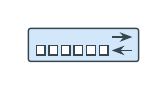
\begin{tikzpicture}[x=1mm,y=1mm,line width=0.5pt]
  \draw[devline, fill=devacc!20, rounded corners=0.8] (0,0) rectangle (14,4.2);
  \foreach \x in {1.0,2.6,...,9.2}{\draw[devline, fill=white] (\x,0.8) rectangle (\x+1.1,2.0);}
  \draw[devline,-{Stealth[length=1.6mm]}] (10.6,3.1) -- (13.2,3.1);
  \draw[devline,-{Stealth[length=1.6mm]}] (13.2,1.4) -- (10.6,1.4);
\end{tikzpicture}}

% --- router -----------------------------------------------------------------------
\newcommand{\devrouter}{%
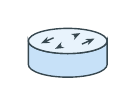
\begin{tikzpicture}[x=1mm,y=1mm,line width=0.5pt]
  \draw[devline, fill=devacc!25] (0,0) -- (0,3) arc[start angle=180,end angle=360,x radius=5,y radius=1.6] -- (10,0) arc[start angle=0,end angle=-180,x radius=5,y radius=1.6] -- cycle;
  \draw[devline, fill=devacc!10] (5,3) ellipse[x radius=5,y radius=1.6];
  \draw[devline,-{Stealth[length=1.1mm]}] (3.2,3.4) -- (1.6,2.7);
  \draw[devline,-{Stealth[length=1.1mm]}] (6.8,2.6) -- (8.4,3.3);
  \draw[devline,-{Stealth[length=1.1mm]}] (4.2,2.4) -- (3.4,2.0);
  \draw[devline,-{Stealth[length=1.1mm]}] (5.8,3.6) -- (6.6,4.0);
\end{tikzpicture}}

% --- firewall (brick wall) -----------------------------------------------------
\newcommand{\devfirewall}{%

\begin{tikzpicture}[x=1mm,y=1mm,line width=0.45pt]
  \fill[devred!25] (0,0) rectangle (10,7.5);
  \foreach \r in {0,1,2,3,4}{%
    \pgfmathsetmacro{\yy}{\r*1.5}
    \draw[devred!70!black] (0,\yy) -- (10,\yy);
    \pgfmathsetmacro{\off}{mod(\r,2)*1.25}
    \foreach \x in {0,2.5,5,7.5}{\pgfmathsetmacro{\xx}{\x+\off}\ifdim\xx pt<10pt \draw[devred!70!black] (\xx,\yy) -- (\xx,\yy+1.5);\fi}}
  \draw[devred!70!black, line width=0.6pt] (0,0) rectangle (10,7.5);
\end{tikzpicture}}

% --- load balancer -----------------------------------------------------------------
\newcommand{\devlb}{%
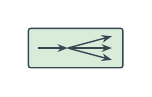
\begin{tikzpicture}[x=1mm,y=1mm,line width=0.5pt]
  \draw[devline, fill=devgreen!20, rounded corners=0.8] (0,0) rectangle (12,5);
  \draw[devline, -{Stealth[length=1.3mm]}] (1.2,2.5) -- (5,2.5);
  \draw[devline, -{Stealth[length=1.3mm]}] (5,2.5) -- (10.6,4.0);
  \draw[devline, -{Stealth[length=1.3mm]}] (5,2.5) -- (10.6,2.5);
  \draw[devline, -{Stealth[length=1.3mm]}] (5,2.5) -- (10.6,1.0);
\end{tikzpicture}}

% --- database (cylinder) ----------------------------------------------------------
\newcommand{\devdb}[1][devacc]{%
\begin{tikzpicture}[x=1mm,y=1mm,line width=0.5pt]
  \draw[devline, fill=#1!20] (0,1.3) -- (0,7.7) arc[start angle=180,end angle=360,x radius=4,y radius=1.3] -- (8,1.3) arc[start angle=0,end angle=-180,x radius=4,y radius=1.3] -- cycle;
  \draw[devline] (0,3.4) arc[start angle=180,end angle=360,x radius=4,y radius=1.3];
  \draw[devline] (0,5.5) arc[start angle=180,end angle=360,x radius=4,y radius=1.3];
  \draw[devline, fill=#1!8] (4,7.7) ellipse[x radius=4,y radius=1.3];
\end{tikzpicture}}

% --- laptop ---------------------------------------------------------------------------
\newcommand{\devlaptop}{%

\begin{tikzpicture}[x=1mm,y=1mm,line width=0.5pt]
  \draw[devline, fill=devline!80, rounded corners=0.5] (1,1.2) rectangle (9,7);
  \fill[devacc!35] (1.7,1.9) rectangle (8.3,6.3);
  \draw[devline, fill=devfill] (0,0) -- (10,0) -- (9,1.2) -- (1,1.2) -- cycle;
\end{tikzpicture}}

% --- desktop workstation ------------------------------------------------------------
\newcommand{\devdesktop}{%

\begin{tikzpicture}[x=1mm,y=1mm,line width=0.5pt]
  \draw[devline, fill=devline!80, rounded corners=0.5] (0,2.4) rectangle (10,9);
  \fill[devacc!35] (0.7,3.1) rectangle (9.3,8.3);
  \draw[devline, fill=devfill] (4.2,2.4) -- (5.8,2.4) -- (6.4,0.6) -- (3.6,0.6) -- cycle;
  \draw[devline, fill=devfill] (2.4,0) rectangle (7.6,0.6);
\end{tikzpicture}}

% --- smartphone -------------------------------------------------------------------------
\newcommand{\devphone}{%

\begin{tikzpicture}[x=1mm,y=1mm,line width=0.5pt]
  \draw[devline, fill=devline!80, rounded corners=0.9] (0,0) rectangle (4.6,8.4);
  \fill[devacc!35] (0.5,1.2) rectangle (4.1,7.4);
  \fill[devfill] (2.3,0.6) circle (0.35);
\end{tikzpicture}}

% --- person (analyst / product team) ---------------------------------------------------
\newcommand{\devperson}[1][devline]{%
\begin{tikzpicture}[x=1mm,y=1mm,line width=0.5pt]
  \fill[#1] (2.5,6.6) circle (1.5);
  \fill[#1] (0,0) -- (0,2.8) arc[start angle=180,end angle=0,radius=2.5] -- (5,0) -- cycle;
\end{tikzpicture}}

% --- cloud (Internet / external API) ------------------------------------------------------
\newcommand{\devcloud}[1][devline!12]{%
\begin{tikzpicture}[x=1mm,y=1mm,line width=0.5pt]
  \node[cloud, cloud puffs=11, cloud puff arc=110, aspect=2.1, draw=devline, fill=#1, minimum width=17mm, minimum height=9mm, inner sep=0pt] {};
\end{tikzpicture}}

% --- GPU / ML inference server ----------------------------------------------------------
\newcommand{\devgpu}{%

\begin{tikzpicture}[x=1mm,y=1mm,line width=0.5pt]
  \draw[devline, fill=devpurple!15, rounded corners=0.6] (0,0) rectangle (6.5,9);
  \draw[devline, fill=white] (0.9,4.6) rectangle (5.6,8.1);
  \foreach \x in {1.5,2.6,3.7,4.8}{\draw[devpurple, line width=0.4pt] (\x,5.0) -- (\x,7.7);}
  \draw[devline, fill=white] (0.9,1.0) rectangle (5.6,3.2);
  \fill[devpurple] (4.6,2.1) circle (0.35);
\end{tikzpicture}}

% --- flag / control-plane server ---------------------------------------------------------
\newcommand{\devflag}{%

\begin{tikzpicture}[x=1mm,y=1mm,line width=0.5pt]
  \draw[devline, fill=devamber!20, rounded corners=0.6] (0,0) rectangle (6.5,9);
  \draw[devline, line width=0.6pt] (1.6,1.2) -- (1.6,8);
  \fill[devamber] (1.6,8) -- (5.4,7.0) -- (1.6,6.0) -- cycle;
  \draw[devline, fill=white] (0.9,1.0) rectangle (5.6,3.0);
\end{tikzpicture}}

% --- ledger (evidence store) ---------------------------------------------------------------
\newcommand{\devledger}{%

\begin{tikzpicture}[x=1mm,y=1mm,line width=0.5pt]
  \draw[devline, fill=devgreen!15, rounded corners=0.5] (0,0) rectangle (9,9);
  \fill[devgreen!45] (0,7) rectangle (9,9);
  \draw[devline] (0,7) -- (9,7);
  \foreach \y in {1.5,3.3,5.1}{\draw[devline, line width=0.3pt] (0.8,\y) -- (8.2,\y);}
  \foreach \x in {3.2,6.0}{\draw[devline, line width=0.3pt] (\x,0.6) -- (\x,7);}
\end{tikzpicture}}

% --- landscapes (utility over configurations) -----------------------------------
\newcommand{\devlandframe}{\draw[devline, fill=white, rounded corners=0.6] (0,0) rectangle (11,7.5);}
\newcommand{\devlandref}{%

\begin{tikzpicture}[x=1mm,y=1mm,line width=0.5pt]
  \devlandframe
  \fill[devacc!22] (0.8,0.8) -- plot[smooth] coordinates {(0.8,1.2) (2.6,2.4) (4.2,4.4) (5.4,6.0) (6.6,4.6) (7.8,5.0) (10.2,1.4)} -- (10.2,0.8) -- cycle;
  \draw[devacc!80!black] plot[smooth] coordinates {(0.8,1.2) (2.6,2.4) (4.2,4.4) (5.4,6.0) (6.6,4.6) (7.8,5.0) (10.2,1.4)};
  \fill[devred] (5.4,6.0) circle (0.55);
\end{tikzpicture}}
\newcommand{\devlandsvc}{%
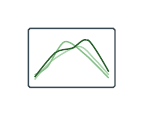
\begin{tikzpicture}[x=1mm,y=1mm,line width=0.5pt]
  \devlandframe
  \draw[devgreen!45] plot[smooth] coordinates {(0.8,1.0) (3.0,3.4) (6.4,5.2) (8.4,3.6) (10.2,1.6)};
  \draw[devgreen!65] plot[smooth] coordinates {(0.8,1.6) (2.4,2.6) (4.6,5.8) (7.2,4.2) (10.2,1.2)};
  \draw[devgreen!60!black] plot[smooth] coordinates {(0.8,1.3) (3.4,4.4) (5.6,5.0) (7.6,6.0) (10.2,2.0)};
\end{tikzpicture}}
\newcommand{\devlandrug}{%

\begin{tikzpicture}[x=1mm,y=1mm,line width=0.5pt]
  \devlandframe
  \fill[devamber!25] (0.8,0.8) -- (0.8,1.6) -- (1.6,3.4) -- (2.3,2.0) -- (3.0,4.6) -- (3.7,2.8) -- (4.5,5.9) -- (5.2,3.3) -- (6.0,5.2) -- (6.7,2.5) -- (7.5,4.8) -- (8.3,3.0) -- (9.1,4.1) -- (10.2,1.5) -- (10.2,0.8) -- cycle;
  \draw[devamber!85!black] (0.8,1.6) -- (1.6,3.4) -- (2.3,2.0) -- (3.0,4.6) -- (3.7,2.8) -- (4.5,5.9) -- (5.2,3.3) -- (6.0,5.2) -- (6.7,2.5) -- (7.5,4.8) -- (8.3,3.0) -- (9.1,4.1) -- (10.2,1.5);
\end{tikzpicture}}

% --- report (results document) ----------------------------------------------------
\newcommand{\devreport}[1][devline]{%
\begin{tikzpicture}[x=1mm,y=1mm,line width=0.5pt]
  \draw[devline, fill=white] (0,0) -- (0,9) -- (5,9) -- (7,7) -- (7,0) -- cycle;
  \draw[devline, fill=devfill] (5,9) -- (5,7) -- (7,7);
  \foreach \y in {5.6,4.3,3.0}{\draw[#1, line width=0.4pt] (1.2,\y) -- (5.8,\y);}
  \draw[devgreen!70!black, line width=0.8pt] (1.3,1.6) -- (2.2,0.9) -- (3.6,2.2);
\end{tikzpicture}}

% --- dice (random scenarios) ------------------------------------------------------
\newcommand{\devdice}{%

\begin{tikzpicture}[x=1mm,y=1mm,line width=0.5pt]
  \draw[devline, fill=devfill, rounded corners=1] (2.2,2.2) rectangle (9.2,9.2);
  \foreach \p in {(3.6,7.8),(7.8,3.6)}{\fill[devline] \p circle (0.6);}
  \draw[devline, fill=white, rounded corners=1] (0,0) rectangle (7,7);
  \foreach \p in {(1.6,1.6),(5.4,5.4),(3.5,3.5),(1.6,5.4),(5.4,1.6)}{\fill[devred] \p circle (0.6);}
\end{tikzpicture}}
